% Created 2026-07-09 Thu 22:56
% Intended LaTeX compiler: pdflatex
\documentclass[presentation]{beamer}
\usepackage[utf8]{inputenc}
\usepackage[T1]{fontenc}
\usepackage{graphicx}
\usepackage{longtable}
\usepackage{wrapfig}
\usepackage{rotating}
\usepackage[normalem]{ulem}
\usepackage{amsmath}
\usepackage{amssymb}
\usepackage{capt-of}
\usepackage{hyperref}
\usepackage[T1]{fontenc}
\usepackage[utf8]{inputenc}
\usepackage[spanish]{babel}
\usepackage[backend=biber, style=apa]{biblatex}
\addbibresource{/home/eareal/Arquitectura-/bibliography/bibliography.bib}
\titlegraphic{
\includegraphics[height=2cm]{images/logoEpn.jpg}}
\usetheme{Madrid}
\usecolortheme{}
\usefonttheme{}
\useinnertheme{}
\useoutertheme{}
\author{Leonardo Rodriguez, Evan Matango, Henry Luisa, Jonathan Pincay}
\date{}
\title{S12 — Soporte del SO: Memoria Virtual, Máquinas Virtuales y WSL}

\hypersetup{
 pdfauthor={Leonardo Rodriguez, Evan Matango, Henry Luisa, Jonathan Pincay},
 pdftitle={S12 — Soporte del SO: Memoria Virtual, Máquinas Virtuales y WSL},
 pdfkeywords={},
 pdfsubject={},
 pdfcreator={Emacs 27.1 (Org mode 9.3)}, 
 pdflang={Spanish}}
\begin{document}

\maketitle
\begin{frame}{Outline}
\tableofcontents
\end{frame}


\section{Soporte del Sistema Operativo (Sección)}
\label{sec:orgb4b9a69}

\begin{frame}[label={sec:org2ebd472}]{Objetivos del SO (G9, 11, 279)}
\begin{itemize}
\item El sistema operativo (SO) es un programa que controla la ejecución
de aplicaciones y actúa como interfaz entre el usuario y el
hardware.
\item \alert{Comodidad:} Su primer objetivo es hacer que el computador sea más
fácil y cómodo de usar para el usuario final.
\item \alert{Eficiencia:} Su segundo objetivo es administrar los recursos del
sistema de forma eficiente para maximizar su aprovechamiento.
\item Actúa como un mecanismo de control inusual: es un programa que cede
el control del procesador a otras aplicaciones y luego lo recupera
para seguir gestionando el sistema.
\end{itemize}
\end{frame}

\begin{frame}[label={sec:orgc5213d3}]{Funciones del SO relacionadas con memoria (G9, 11, 279)}
\begin{itemize}
\item Existe la  mono pogramacion que se basan en la ejecucion de
un solo proceso hasta que este termine de ejecutarse.
\item La multiprogramacion en cambio trabaja con multiples procesos
consecutivos asignandoles un espacio de memoria y tiempo especificos
para terminar de ejecutarse.
\item \alert{Intercambio (Swapping):} Para evitar que el procesador quede
inactivo, el SO mueve temporalmente al disco los procesos que están
en espera, liberando espacio en memoria principal para nuevos
trabajos.
\end{itemize}
\end{frame}
\begin{frame}[label={sec:org41d3f0a}]{Estados de un Proceso (Planificación)}
\begin{center}
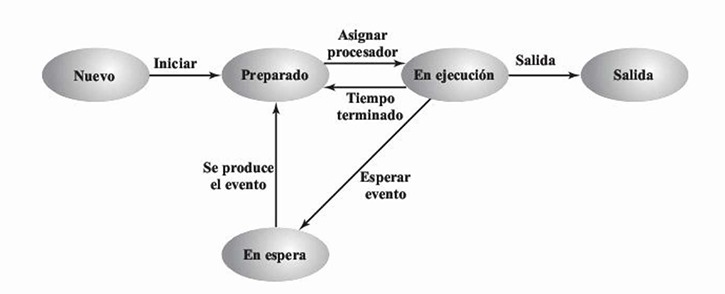
\includegraphics[width=0.85\textwidth]{images/Procesos.png}
\end{center}
\end{frame}
\section{Planificación y Memoria Virtual (Sección)}
\label{sec:org2b437dd}

\begin{frame}[label={sec:org85f46e5}]{Planificación de la memoria (G9, 11, 280)}
\begin{itemize}
\item \alert{Particionamiento:} Puede ser fijo (tamaños predefinidos) o dinámico
(asignación exacta requerida). Ambos métodos generan espacios
desperdiciados o fragmentación con el tiempo.
\item \alert{Paginación:} El SO divide la memoria en marcos de tamaño fijo y los
procesos en páginas.
\item \alert{Segmentacion:} El SO divide la memoria en partes de tamaño variable
y tambien los procesos en segmentos con diferentes tipos de
funciones como las principales y las secundarias.
\end{itemize}
\end{frame}

\begin{frame}[label={sec:org252f7d0}]{Principios de Memoria Virtual (G9, 11, 282)}
\begin{itemize}
\item Permite ejecutar un proceso sin cargar todas sus instrucciones y
datos en la memoria principal de manera simultánea.
\item \alert{Paginación por demanda:} Las páginas se traen a la memoria solo
cuando se solicitan explícitamente, aprovechando el principio de
localidad.
\item El programador percibe un espacio de memoria enorme (memoria virtual
en disco) sin preocuparse por los límites de la memoria real
(RAM).
\end{itemize}
\end{frame}

\begin{frame}[label={sec:orgddaddab}]{Paginación (G9, 11, 283)}
\begin{columns}
\begin{column}{0.5\columnwidth}
\begin{itemize}
\item La memoria física se divide en trozos fijos llamados \alert{marcos} (frames).
\item Los procesos se dividen en \alert{páginas} del mismo tamaño.
\item La tabla de páginas mapea cada página virtual a su marco físico.
\item Minimiza el desperdicio de memoria.
\end{itemize}
\end{column}

\begin{column}{0.5\columnwidth}
\begin{center}
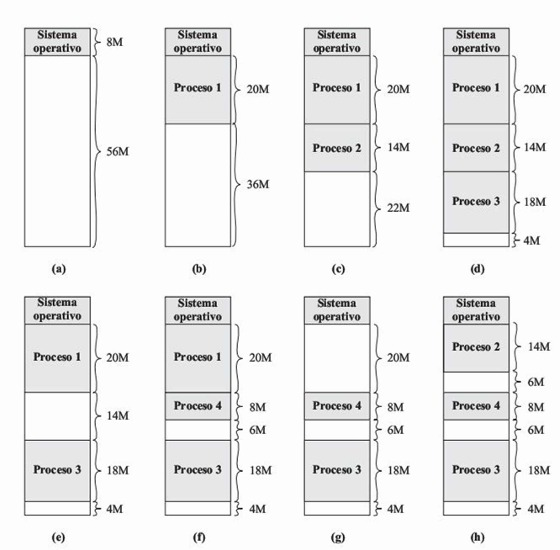
\includegraphics[width=0.9\textwidth]{images/figura_8_14.png}
\end{center}
\end{column}
\end{columns}
\end{frame}
\section{Traducción de Direcciones (Sección)}
\label{sec:org34a640a}

\begin{frame}[label={sec:org243184f}]{Traducción de direcciones virtuales a físicas (G9, 11, 285)}
\begin{columns}
\begin{column}{0.5\columnwidth}
\begin{itemize}
\item Direcciones lógicas: Número de página + desplazamiento.
\item Direcciones físicas: Marco de página + desplazamiento.
\item La CPU usa la tabla de páginas del proceso actual para hacer la traducción en tiempo real.
\end{itemize}
\end{column}

\begin{column}{0.5\columnwidth}
\begin{center}
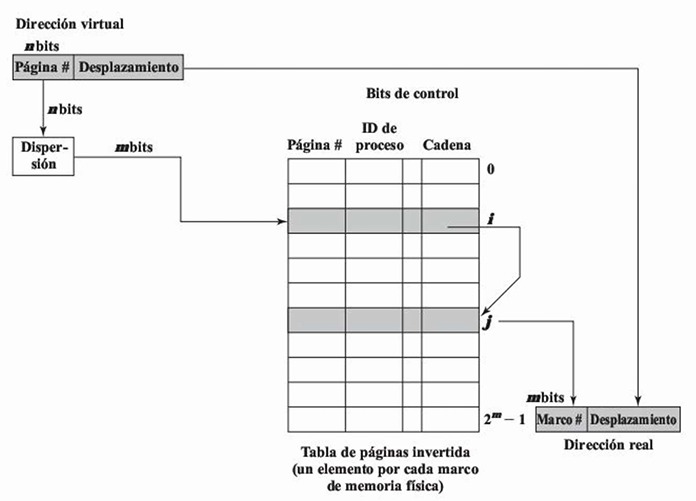
\includegraphics[width=\textwidth]{images/traduccion_direcciones.png}
\end{center}
\end{column}
\end{columns}
\end{frame}
\begin{frame}[label={sec:org8c3a379}]{TLB (Translation Lookaside Buffer) (G9, 11, 287)}
\begin{itemize}
\item Toda referencia a memoria virtual implicaría dos accesos (uno a la
tabla de páginas y otro al dato), reduciendo el rendimiento a la
mitad.
\item El TLB soluciona esto actuando como una caché especial de alta
velocidad que almacena las entradas de la tabla de páginas usadas
más recientemente.
\item Si hay un acierto en el TLB, la dirección física se genera de
inmediato sin necesidad de consultar la tabla de páginas alojada en
la memoria RAM.
\end{itemize}
\end{frame}

\begin{frame}[label={sec:org17166fd}]{Page Faults y reemplazo de páginas (G9, 11, 290)}
\begin{itemize}
\item Si el procesador intenta acceder a una página que actualmente no se
encuentra en la memoria principal, se produce un \alert{fallo de página}.
\item El sistema operativo interviene, trae la página solicitada desde el
almacenamiento masivo (disco) y actualiza la tabla de páginas.
\item \alert{Reemplazo:} Si la memoria está llena, el SO debe predecir y sacar
la página con menor probabilidad de uso futuro, evitando que el
procesador pase todo su tiempo intercambiando páginas
(hiperpaginación).
\end{itemize}
\end{frame}
\section{Máquinas Virtuales (Sección)}
\label{sec:org973cf68}

\begin{frame}[label={sec:org838dfb6}]{Concepto de Máquina Virtual (G9, 11, 292)}
\begin{itemize}
\item Una máquina virtual (VM) abstrae el hardware físico de un computador
para que múltiples sistemas operativos puedan compartir los mismos
recursos de forma simultánea.
\item \alert{Host OS:} Es el sistema operativo físico subyacente que controla el
hardware real.
\item \alert{Guest OS:} Es el sistema operativo virtualizado que se ejecuta
dentro de la máquina virtual creyendo que tiene acceso exclusivo al
hardware.
\end{itemize}
\end{frame}

\begin{frame}[label={sec:orgd984d66}]{Hipervisores: Tipo 1 y Tipo 2 (G9, 11, 295)}
\begin{columns}
\begin{column}{0.4\columnwidth}
\begin{itemize}
\item \alert{Tipo 1 (Bare Metal):} Se ejecuta directo en el hardware (ej. ESXi). Máximo rendimiento.
\item \alert{Tipo 2 (Hosted):} Es una aplicación sobre el SO anfitrión (ej. VirtualBox).
\item El hipervisor multiplexa CPU, memoria y E/S.
\end{itemize}
\end{column}

\begin{column}{0.6\columnwidth}
\begin{center}
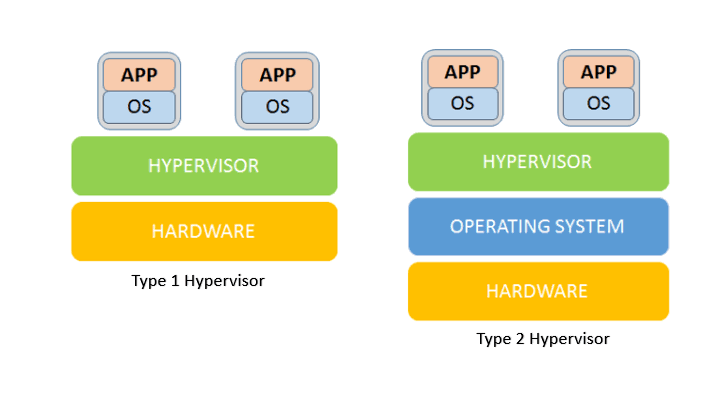
\includegraphics[width=\textwidth]{images/hipervisores.png}
\end{center}
\end{column}
\end{columns}
\end{frame}
\begin{frame}[label={sec:org2686011}]{Virtualización de memoria (G9, 11, 298)}
\begin{itemize}
\item Añade un nivel extra de complejidad en la traducción: el Guest OS
traduce direcciones virtuales a "direcciones físicas virtuales".
\item El hipervisor debe atrapar estas peticiones y traducir las
direcciones físicas virtuales a las verdaderas direcciones físicas
reales de la máquina anfitriona.
\item Se utilizan técnicas de hardware integradas en la CPU (como Shadow
Page Tables o soporte Intel EPT / AMD-V) para acelerar drásticamente
este doble mapeo.
\end{itemize}
\end{frame}
\section{WSL como caso de estudio (Sección)}
\label{sec:orgfc13bf6}

\begin{frame}[label={sec:org98619b9}]{Windows Subsystem for Linux (WSL) (G9, 11, 301)}
\begin{itemize}
\item WSL es una característica de Windows que permite a los desarrolladores ejecutar un entorno GNU/Linux (herramientas CLI, utilidades y aplicaciones) de forma nativa.
\item Evita el sobrecoste de recursos y los tiempos de arranque lentos asociados a una máquina virtual tradicional completa.
\item Facilita el desarrollo cruzado sin necesidad de reiniciar la computadora (dual-boot).
\end{itemize}
\end{frame}

\begin{frame}[label={sec:orgd26eafb}]{WSL1 vs WSL2: arquitectura (G9, 11, 303)}
\begin{columns}
\begin{column}{0.4\columnwidth}
\begin{itemize}
\item \alert{WSL1:} Capa de traducción de llamadas al sistema (Linux a NT). No hay kernel real.
\item \alert{WSL2:} Máquina virtual ligera altamente optimizada.
\item Ejecuta un kernel de Linux completo mejorando el rendimiento de E/S.
\end{itemize}
\end{column}

\begin{column}{0.6\columnwidth}
\begin{center}
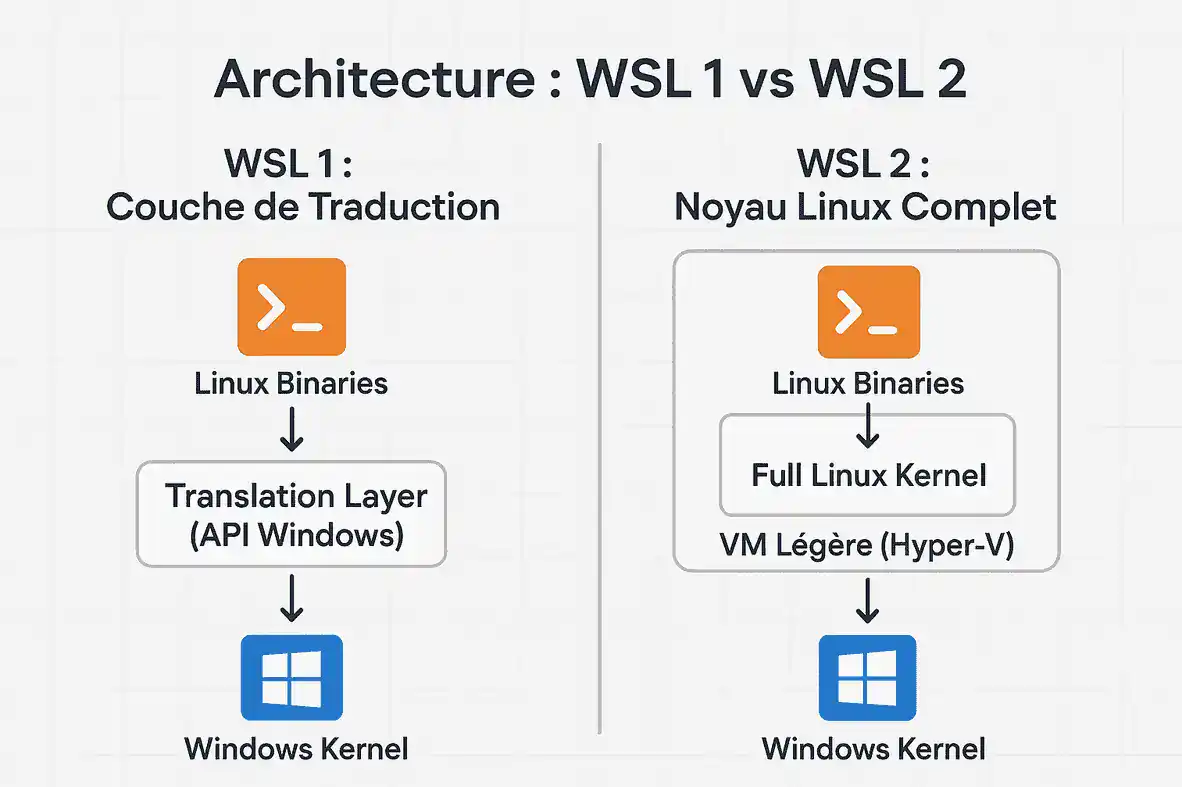
\includegraphics[width=\textwidth]{images/arquitectura_wsl.png}
\end{center}
\end{column}
\end{columns}
\end{frame}
\begin{frame}[label={sec:org58f3c32},fragile]{Integración con el sistema de archivos Windows (G9, 11, 305)}
 \begin{itemize}
\item WSL permite acceder a los discos de Windows (C:, D:) desde Linux montándolos automáticamente en el directorio \texttt{/mnt/}.
\item WSL2 utiliza un disco duro virtual (VHD) con formato nativo \texttt{ext4} para el sistema de archivos raíz de Linux.
\item El acceso y la transferencia de archivos cruzada entre ambos sistemas operativos se realiza mediante el protocolo de red 9P.
\end{itemize}
\end{frame}

\begin{frame}[label={sec:orgc6a4aaf}]{WSL y memoria virtual (G9, 11, 307)}
\begin{itemize}
\item A diferencia de las VMs de Tipo 2 tradicionales que reservan y
bloquean un fragmento estático de RAM, la VM de WSL2 asigna y libera
memoria dinámicamente según la demanda.
\item Si Linux libera memoria de su caché interna, WSL2 se encarga de
devolver esa memoria RAM física al Host (Windows) para que otras
aplicaciones de escritorio puedan utilizarla.
\end{itemize}
\end{frame}
\section{Referencias}
\label{sec:orgd7f9340}
\begin{frame}[allowframebreaks]{Bibliografía}
\printbibliography
\end{frame}

\section{Indicaciones}
\label{sec:org9d45242}
\begin{frame}[fragile,allowframebreaks]{Indicaciones}
 \begin{itemize}
\item Recuerde que si \texttt{options: H:2}, entonces:
\begin{itemize}
\item \texttt{*} Declara el nombre de la Sección
\item \texttt{**} Declara el nombre de la diapositiva
\end{itemize}
\item Puede alterar la estructura de la diapositiva si lo considera necesario
\item Para este tema consulte las siguientes fuentes:
\begin{itemize}
\item \textcite{stallings2022computer}, 11ava edición, 2022, English,
capítulo 8: Operating System Support, páginas 279 a 314.
\item \textcite{stallings2006esp}, 7ma edición, 2006, Español,
capítulo 8: Soporte del Sistema Operativo.
\end{itemize}
\item El grupo G9 expone este tema.
\item El grupo expone el tema y sube la presentación (\texttt{.ORG} y \texttt{.PDF} para Beamer, o \texttt{.ORG} y \texttt{.HTML} para reveal.js)
\item El grupo sube las ayudas memoria/notas del tema usando la plantilla \url{FormatoTareas/TemplateNotasClase.org} (\texttt{.ORG} y \texttt{.PDF})
\end{itemize}
\end{frame}
\end{document}
